\documentclass[12pt]{beamer}

\usepackage{amsmath}
\usepackage{float}
\usepackage{graphicx}
\usepackage[utf8]{inputenc}

\mode<presentation>{\usetheme{Madrid}}
\title{Difracción de Franhaufer}
\author{Alfredo Ricci y Juan Andrés Urrea}

\begin{document}
%La portada
\frame{\titlepage}
%Así se comienza cada diapositiva
\begin{frame}
\frametitle{Para desarrollar...}
\begin{block}{}
\begin{enumerate}
\item Introducción y Marco Teórico \pause
\item Simulaciones Preliminares \pause
\item Montaje Realizado \pause
\item Datos Recolectados y Análisis \pause
\item Conclusiones
\end{enumerate}
\end{block}
\end{frame}

%La introducción
\begin{frame}
\frametitle{Introducción}
\begin{block}{}
\begin{itemize}
\item Se elige este tema por interés del grupo... \pause
\item Forma interesante de mezclar aspectos matemáticos y fenómenos observables... \pause
\item Forma didáctica de abordar la transformada de Fourier...
\end{itemize}
\end{block}
\end{frame}

%Marco Teórico
\begin{frame}
\frametitle{Marco Teórico}
\end{frame}

%Montaje
\begin{frame}
\frametitle{Montaje Utilizado}

\begin{figure}[htb]
\centering
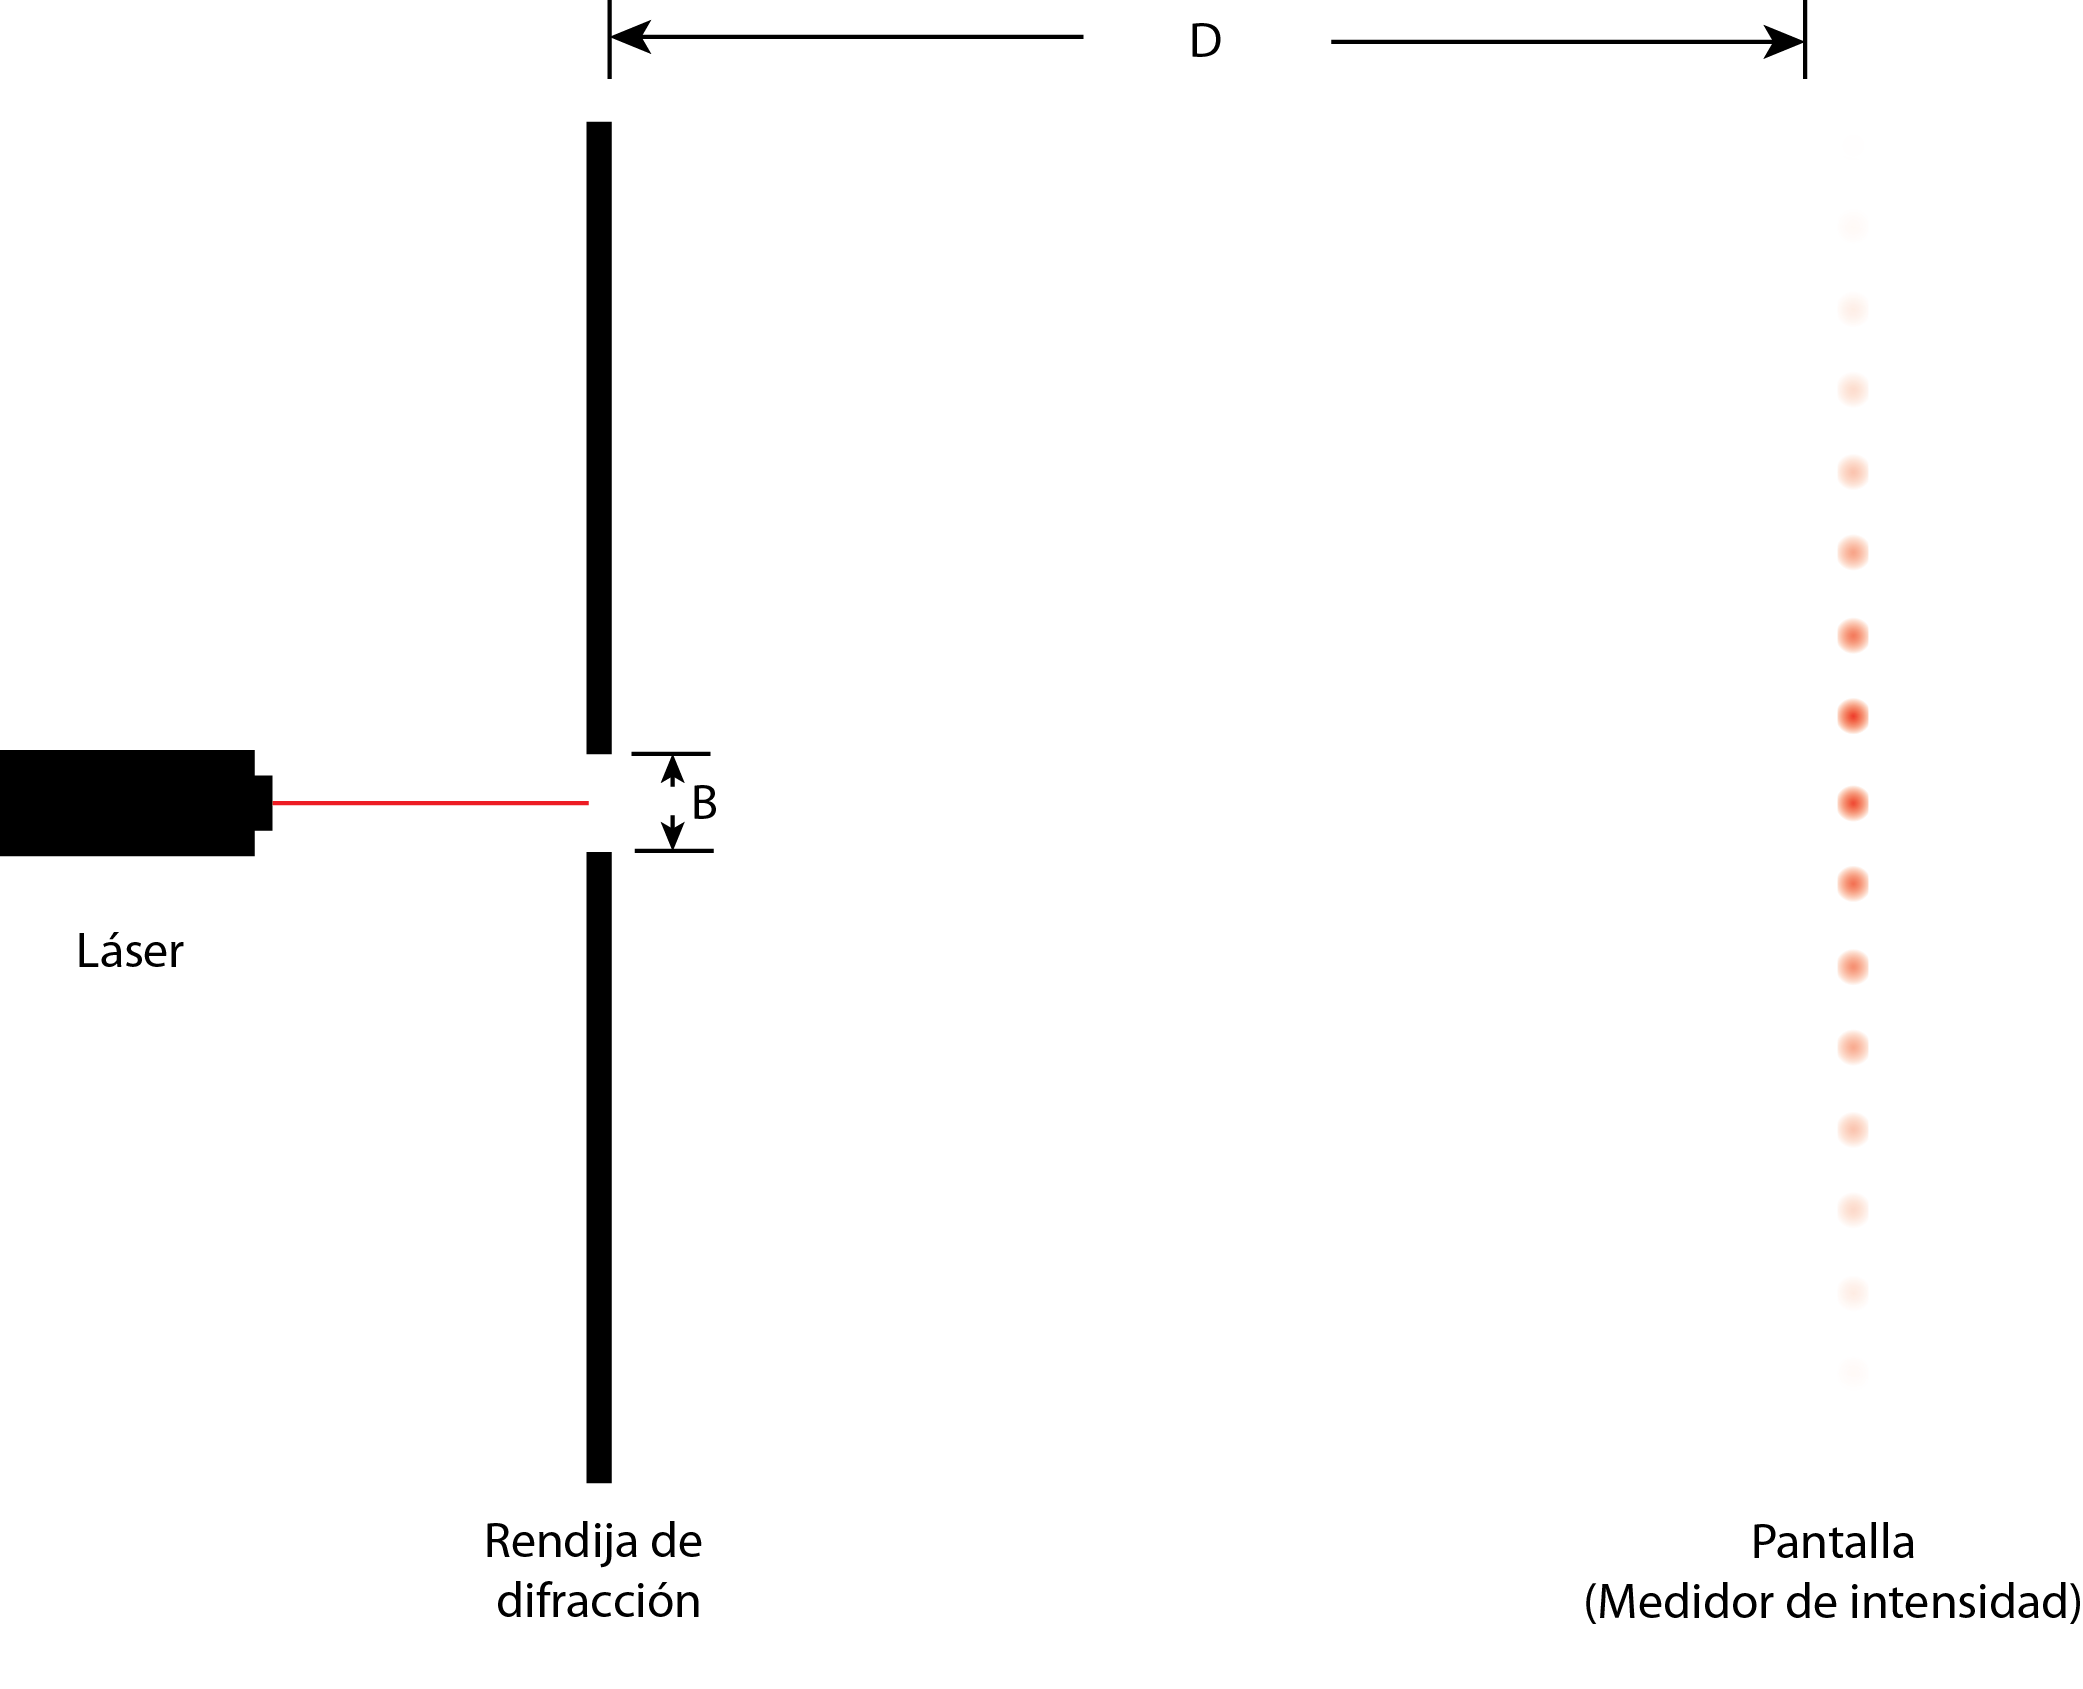
\includegraphics[width=0.4\textwidth]{Montaje.png}
\caption{Montaje a Construir} \label{fig:montaje}
\end{figure}
\end{frame}
\end{document}

